
\section{Quasi-SERDES Physical Link Module}
\subsection{Quasi-SERDES Physical Link Module Block Schematic}
\begin{frame}
\frametitle{Quasi-SERDES Physical Link Module Input/Output Port}
This Quasi-SERDES Physical link module is a partial serializer / de-serializer block which can be used as and interface between two routers.\\
	\centering
	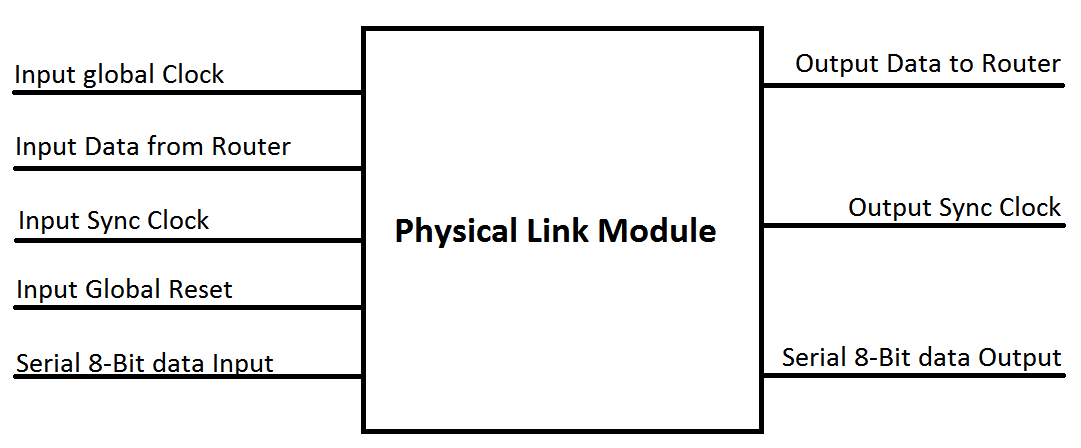
\includegraphics[scale=0.35]{./figs/physicalModule}
\end{frame}

\begin{frame}
\frametitle{Quasi-SERDES Physical Link Module Input/Output Port}
\small
\begin{center}
\begin{tabular}{||c | c||} 
\hline
\textbf{PIN} & \textbf{DESCRIPTION} \\ \hline
CLK & Input Clock \\
rst\_n & Global Reset Input(Active low Reset)\\
input\_data\_from\_router[17:0] & 18 bit input Flit\\
serial\_data\_in[7:0] & 8 bit data input (MSB first)\\
serial\_data\_out[7:0] & 8 bit data output (MSB first)\\
output\_data\_to\_router[17:0] & Reconstructed Flit \\
sync\_clk\_in & input synchronization clock \\
sync\_clk\_out & output synchronization clock \\
\hline
\end{tabular}
\end{center}
\end{frame}


\begin{frame}
\frametitle{Features}
\begin{itemize}
\item Clock synchronization and reset synchronization is handled in the module
\item Any bit to 8-bit serialization/de-serialization
\item Data reconstruction with validity check
\item Flow control to ensure lossless data exchange
\item Simple GPIO to GPIO full duplex communication interface
\item 2 $\times$ 2 $\times$ n bit (data) / 8 - gives the number of clock cycles for data transfer. Therefore for 24 bit input data we need 12 clock cycles, so effectively 2 bits/clock
\item Therefore, if clock is 50MHz (tested on DE0-Nano), Data-rate is 100Mbps
\item Buffer-full indication to routers to stop it from sending flits
\end{itemize}
\end{frame}

